 \documentclass{beamer}
\usefonttheme{professionalfonts}
\usepackage{agda}
\usepackage{catchfilebetweentags}
\usetheme{CambridgeUS}
\usecolortheme{seahorse}

\usepackage{amssymb}
\usepackage{bbm}
\usepackage[greek,english]{babel}

\beamertemplatenavigationsymbolsempty

\title{Musical Ornaments}
\author{John Leo}
\institute{Halfaya Research}
\date{May 14, 2018}
 
\begin{document}
 
\frame{\titlepage}
 
\begin{frame}\frametitle{Outline}
\begin{itemize}
\item A look toward the future
\item Music Tools
\item Equivalences and Ornaments
\end{itemize}

\bigskip 
Sources:
\begin{itemize}
\item {\tt https://github.com/halfaya/MusicTools}
\end{itemize}
\end{frame}

\begin{frame}\frametitle{Robert Harper}
\begin{quote}
Eventually all the arbitrary programming languages are going to be just swept away with the oceans,
and we will have the permanence of constructive, intuistionistic type theory as the master theory
of computation---without doubt, in my mind, no question.  So, from my point of view---this is a personal
statement---working in anything else is a waste of time.
\end{quote}

CMU Homotopy Type Theory lecture 1, 52:56--53:20.
\end{frame}

\begin{frame}\frametitle{What will programming look like in 50 years?}
\begin{itemize}
\item Convergence of math and computer science
\item Functional Programming, Algebra of Programming
\item Dependent Types or a successor (Cubical?)
\item Who does the programming?
\end{itemize}
\end{frame}

\begin{frame}\frametitle{How do we get there from here?}
\begin{itemize}
\item Add dependent types to an industrial-strength language (Haskell)
\item Make a dependently typed language (Agda, Idris) practical to use
\item Learn how to program using dependent types
\item Many theoretical and practical advances are still needed
\end{itemize}
\end{frame}


\begin{frame}\frametitle{Euterpea}
\begin{figure}
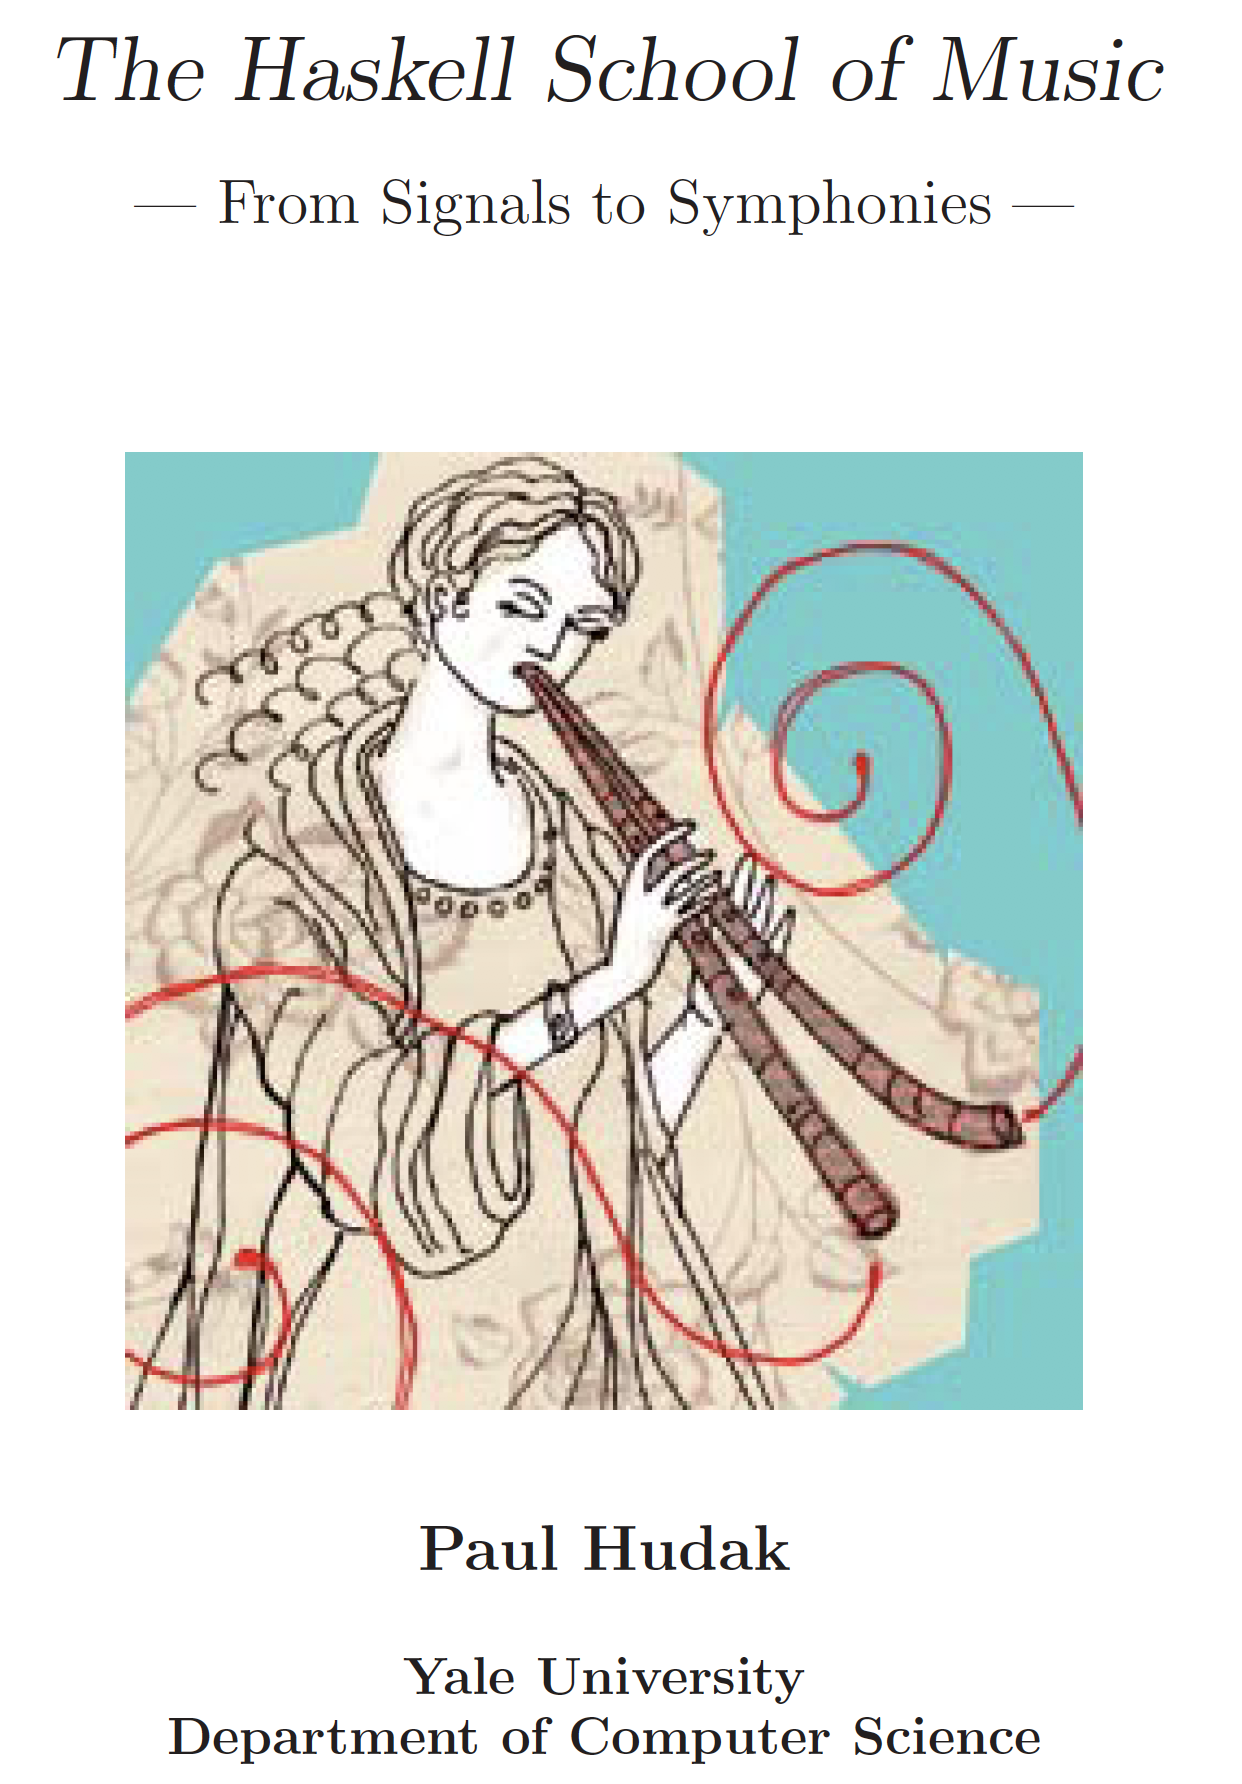
\includegraphics[height=0.8\textheight]{hsom}
\end{figure}
\end{frame}

\begin{frame}\frametitle{Music Tools}
\begin{itemize}
\item Collection of composable tools for synthesis and analysis of music
\item Originally written in Haskell
\item Converted to Agda, using Haskell for MIDI interface
\item Explore programming using dependent types in a circumscribed yet rich domain
\item Use math, including transport of equivalences (from HoTT) and Ornaments
\end{itemize}
\end{frame}

\begin{frame}\frametitle{Look vs Time (1997)}
\begin{figure}
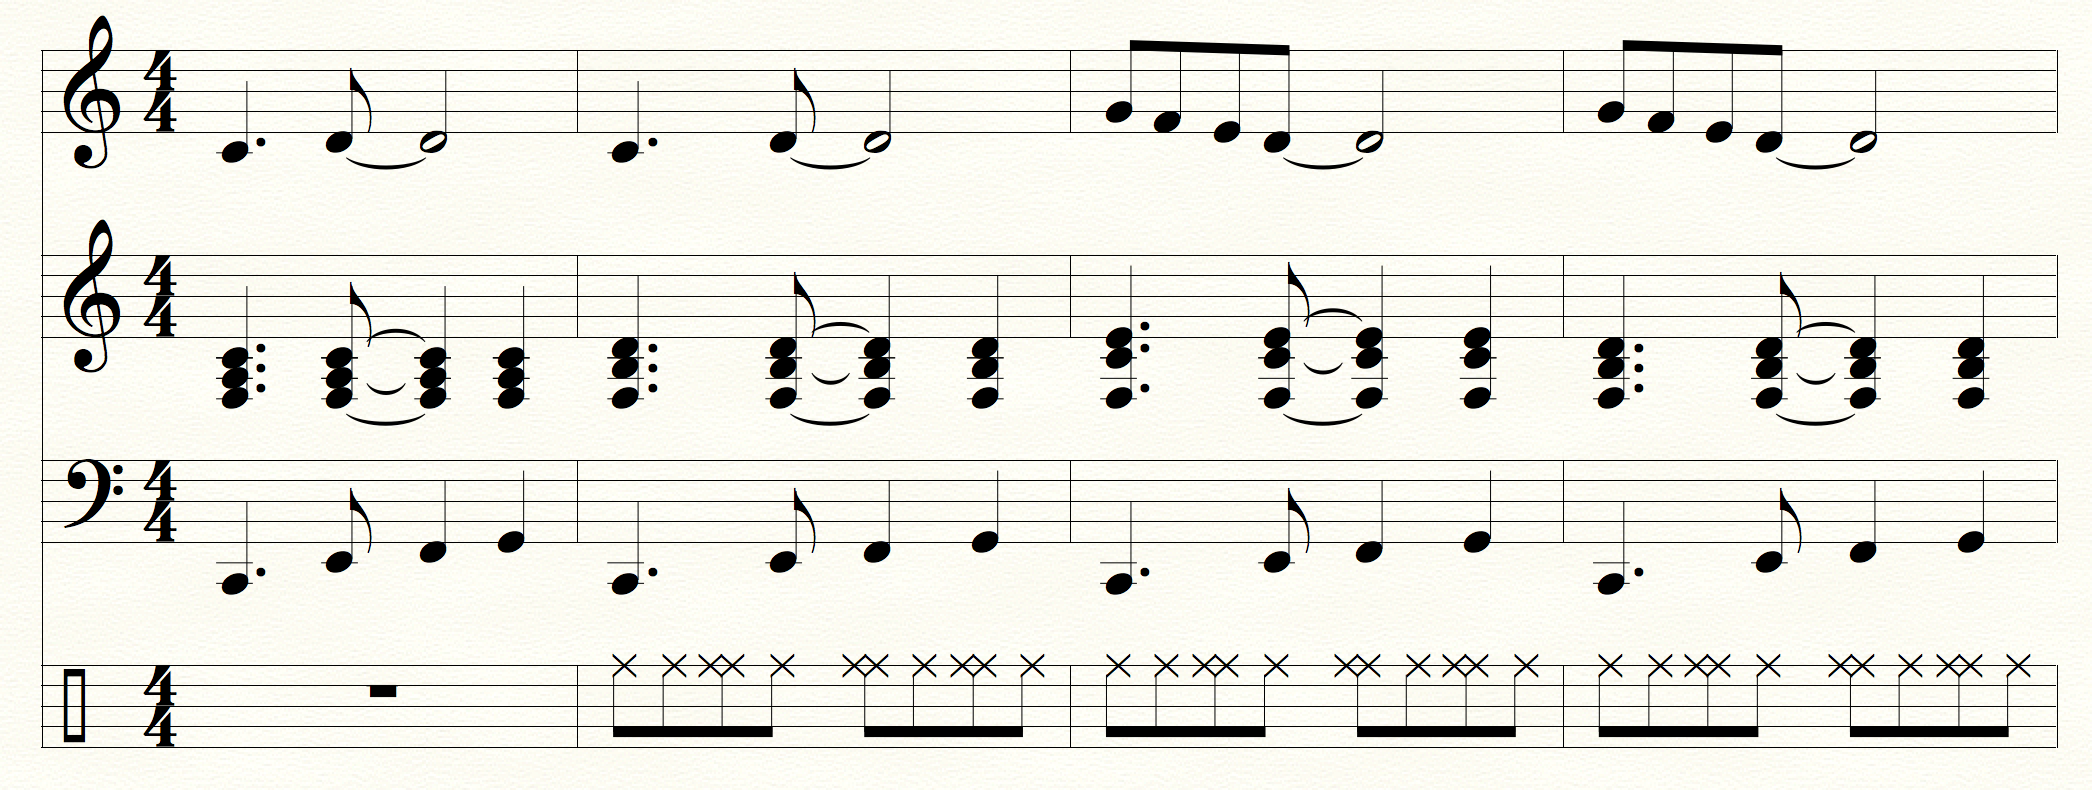
\includegraphics[width=\textwidth]{lookVsTime}
\end{figure}
\end{frame}

\begin{frame}\frametitle{Music Representation \`a la Euterpea}
\ExecuteMetaData[../agda/latex/Pnwplse.tex]{pitch}
\ExecuteMetaData[../agda/latex/Pnwplse.tex]{duration}
\ExecuteMetaData[../agda/latex/Pnwplse.tex]{note}
\ExecuteMetaData[../agda/latex/Pnwplse.tex]{music}
\end{frame}

\begin{frame}\frametitle{Equivalent Representations of Pitch}
\ExecuteMetaData[../agda/latex/Pnwplse.tex]{pitch}
\ExecuteMetaData[../agda/latex/Pnwplse.tex]{chromatic}
\ExecuteMetaData[../agda/latex/Pnwplse.tex]{relpitch}
\ExecuteMetaData[../agda/latex/Pnwplse.tex]{octave}
\ExecuteMetaData[../agda/latex/Pnwplse.tex]{pitchoctave}
\end{frame}

\begin{frame}\frametitle{Equivalences}
\begin{itemize}
\item Define an equivalence between {\tt Pitch} and {\tt PitchOctave}
\item Using HoTT techniques, automatically lift this equivalence to functions defined using \texttt{Pitch}
\item See \textit{Equivalences for Free!} (Tabareau, Tanter, Sozeau)
\item Challenge: Defining base equivalences. Can this be automated?
\end{itemize}
\end{frame}

\begin{frame}[fragile]\frametitle{Ornaments}
\begin{semiverbatim}
data Music a  = ... 
  |  Modify Control (Music a)

data Control = ...
  |  Phrase [PhraseAttribute]

data PhraseAttribute = ...
  |  Orn Ornament

data Ornament =
  Trill | Mordent | InvMordent | DoubleMordent |
  Turn | TrilledTurn | ShortTrill ...
\end{semiverbatim}
\end{frame}

\begin{frame}\frametitle{Ornaments}
\begin{itemize}
\item Functions on a base {\tt Music} structure can be automatically lifted to operate on {\tt Music} ornamented with additional information
\item See works on Ornaments by McBride, Dagand and others
\item Challenge: Shallow embedding of ornaments in Agda
\end{itemize}
\end{frame}

\begin{frame}\frametitle{Conclusion}
\begin{itemize}
\item Music is a good domain in which to explore  practical application of dependent types
\item Using math can be more work at first, but should be a big win in the long term
\item Figure out how to minimize the work and maximize the reward
\end{itemize}
\end{frame}

\end{document}
